\documentclass[12pt,letterpaper]{article}
\usepackage[latin1]{inputenc}
\usepackage{amsmath}
\usepackage{amsfonts}
\usepackage{amssymb}
\usepackage[margin=1in]{geometry}
\usepackage{graphicx}

\graphicspath{ {./} }

\author{Ben Kahan}
\title{DS 210: Final Project Report}

\begin{document}

\maketitle

\pagebreak

\section{Introduction}

This project aimed to explore connectivity between directors of the 5000 movies,  ranked by IMDB.  The data set consists of multiple genres across a very large time span: 1920s to Present (2022).  The data set is sourced from Kaggle.com and is titled: "IMDb 5000+ Movies \& Multiple Genres Dataset".  

The project's language is Rust and the entirety of the project was completed solely by Ben Kahan.  The chosen VCS is git and the project's repository is hosted on GitHub.  I edited and debugged using IntelliJ IDEA (Ultimate Edition) with the Rust plugin. 

\section{Data Intake and Organization}

This presented a challenged I did not expect.  When I selected my data set, I had initially had ideas on how to turn this data into graph data.  Initially, I imported and reused my code from Homework 10. However,  I quickly realized that I would need a custom implementation in order to work with my data.  

Originally, I created a struct called \texttt{NodeData}.  This contains all the important information for each line in the data CSV file. 

\subsection{What is Important Data?}

From the header of the data file:

\begin{verbatim}
Movie_Title
Year
Director
Actors
Rating
Runtime(Mins)
Censor
Total_Gross
main_genre
side_genre

\end{verbatim}
I removed: \texttt{Censor, Rating, Total\_Gross}

These were selected as I did not require censorship information about the movies nor was I interested in the rating and gross income of each movie. 

I was looking for sub-graphs and networks that describe the hidden relationships of actors and and their movies.  I believe that \texttt{Rating} and \texttt{Censor} are not required for this analysis and I chose to omit \texttt{Total\_Gross} due to time. 

To aid my decision, I opened the data set in a Jupyter Notebook and inspected the CSV file's features. The notebook is included in addition to all Rust files. 

\subsection{My Idea}

My idea was to create a "2D graph" and I thought that I would be able to implement it in a similar fashion to Red/Black Trees. (i.e., by labeling). I wanted to construct a graph that was connected via Actor/Actresses but centered around Individual movies. For instance,  since Adam Sandler is in 50 First Dates and Grown Ups, the two movies would be connected by Adam Sandler.  

I would create this graph by indexing every actor/actress in every movie in the data set (yes, very expensive). Then, I would connect them by adding each movie in a vector.  This would connect movies by means of actors. 

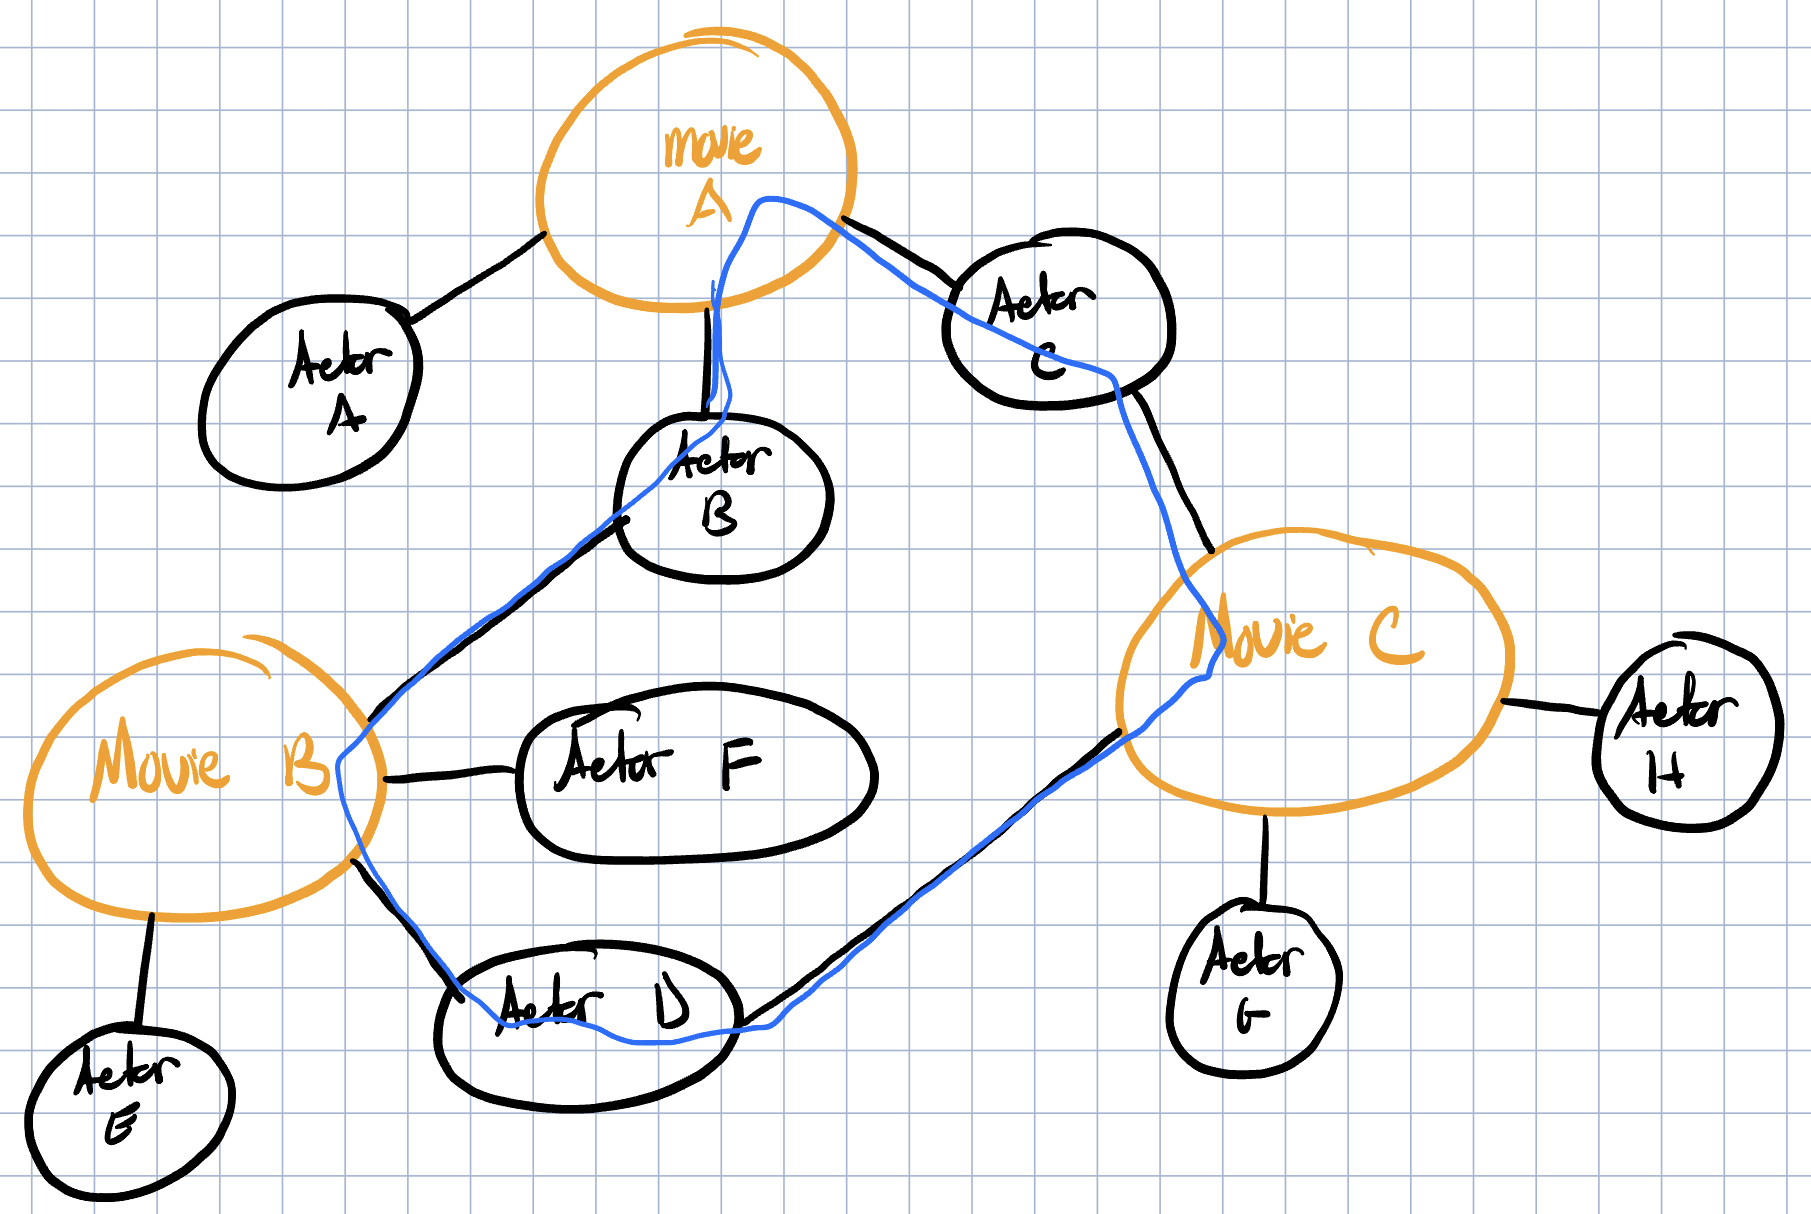
\includegraphics[scale=.24]{draft-graph.jpeg}

However,  this was significantly harder to implement than expected.  I thought that it would be straight forward to adapt full-connected graph algorithms to n-graphs but I was proven wrong.  


\subsection{Data Structure Issues}

I worked with this version of \texttt{NodeData} but I was originally confused on how I would exactly implement a graph for this data. Initially, I created a double vector containing \texttt{NodeData} structs.  

This, however, proved to be an unsuccessful attempt and it would keep me stuck in a loop for over a week. 

I did not do my diligence when I began the project and I did not draw my plan to implement. Thus,  I spent many hours working on code that would not fundamentally work for my data. 

My original code worked approximately like this: 

\begin{enumerate}
\item Read in CSV,  convert to \texttt{vec<NodeData>}
\item Create a graph object with adjacency list: \texttt{Vec$<$\&Vec$<$\&NodeData$>>$}
\item Insert data into the graph:
	\begin{enumerate}
		\item Count the number of actors by iterating through each \texttt{NodeData} (very inefficient and messy) 
		\item Hash the name of each actor,  modded with the length of the adjacency list
		\item Push \texttt{NodeData} onto the vector from \texttt{graph.get(hash(actor)).push(NodeData)}
	\end{enumerate}

\end{enumerate}

This presented numerous problems when I tried to do analysis of the data.  When implemented breadth-first search, I realized that I was, on occasion,  getting hash collisions. I determined that this would not an issue with Rust, rather it was most likely due to my handling of the data and I must have confused myself.  Since the code wasn't optimized, I had to convert back and forth between compatible data types (for instance, \texttt{i16} to \texttt{usize}). 

I then decided to rewrite and reorganize the majority of my code.  I began my adjusting the data structure of the graph. 

Where I originally used nested vectors,  I decided to use \texttt{HashMap<key: Actor as String, value: Vec<NodeData>}.  This allowed me to uniquely match strings and connect actors to movies and vice versa. 

\section{Data Analysis}

\subsection{Where's the Analysis?}

Unfortunately,  this is nearly as far as I got.  Due to factors mainly within my control,  I did not start working on this project until after Thanksgiving and I did not actively work on it until early December.  I overestimated my abilities and underestimated my knowledge of the Rust language.  I believed that my prior experience with graph data structures and algorithms would help me in this project but I underestimated how much programming knowledge I had lost since taking that class (CSC 172-173 at the University of Rochester, if you're interested). In addition, the majority of my formal programming experience was in Java and C-- both languages that are too similar to Rust to make Rust easy, in my opinion. However, I did learn many new things about Rust. 

\subsubsection{Rust versus Every Other C-based Language,  A Student's Perspective}
\begin{itemize}
	\item Write Rust code like you need to ask for consent, everything needs to explicitly stated 
	\item Memory is incredibly safe 
	\item The compiler is your friend,  build to get latest updates on your code 
	\item Make sure Cargo Check is running! 
	\item Everything seems harder to do in Rust because of the first point 
	\item Rust is more like Java but with Python semantics   
	\item Rust is really fast and portable 
\end{itemize}


\subsection{Attempted Analysis}

Once I had created the graph data structure, I needed to make sure that it actually worked.  I figured that the easiest way to do this was to print the graph actor by actor. 

\subsubsection{Simple "Traverse"}

I wrote a simple function to print out each \texttt{NodeData} for each actor.  The function is called \texttt{fn print\_graph(graph: \&Graph)}

\subsubsection{Breadth-First Search: Incomplete}

I used the Wikipedia version of the pseudo-code to derive my own implementation of the search. I had to modify the pseudo-code as I (most likely) had a disconnected graph so the standard implementation would miss some vertices.  The function is called \texttt{fn bfs(graph: \&Graph)}

I hinted about this above but this is where I failed to properly traverse the graph. The code that I have commented out will not compile and run but I believe that I am getting closer to the solution. 

\section{Conclusion}

\subsection{The Remainder of the Plan}

For the rest of the project,  I was hoping to do a mini-EDA and build the tools needed along the way.  I was hoping to get statistics using total gross income, connection between directors and actors, etc. All of this appeared like a straightforward and simple task but I overestimated my capabilities.  

\subsection{My Performance}

I did not do nearly as much as I wanted to do on this project.  I know that I will receive an unsatisfactory grade but that is the result of my own doings.  As I have previously stated in this report,  I underestimated this project and overestimated my abilities.  I give myself a small break as I hop worlds between my job, my business, and school.  That said, I had many goals in mind. I wanted to explore connectivity in the graph. Since the movies are connecting the actors, there's significant meaning to connectivity. Like social networks,  the graph visually explains trends in actors (and by abstraction, genres) through time. 

Since movies and thus, actors, are all time-series elements, there's an additional layer to the graph.  This is one aspect that continues to trouble my mind as the graph contains many different \textit{layers}, each of them unique.  

All said, I accept my grade on this project and I hope to improve on my future projects as this is leaving me quite disappointed in myself.  This project made it clear that I need to set more explicit (and realistic) time-lines.  Throughout this semester, it became very clear to me that I prefer to work alone.  I know that many of problems would likely have been solved had I gone office hours and conversed with my classmates. 

\subsection{Opinions on Rust}
This class leaves me with questions regarding my own opinions on Rust in the data science space. I've concluded that I see the usefulness and necessity of a language like Rust but it's safety is also a hindrance.  I found that, while Rust creates fast code, it doesn't appear to be as suited as Python (\texttt{Numpy, SKLearn, Pandas)}, Julia, or R.  

However, I do believe that Rust is a wonderful solution for production codebases and I suspect that support will scale as the language matures. 


\end{document}